%% LyX 2.0.3 created this file.  For more info, see http://www.lyx.org/.
%% Do not edit unless you really know what you are doing.
\documentclass[twoside,english]{paper}
\usepackage{lmodern}
\renewcommand{\ttdefault}{lmodern}
\usepackage[T1]{fontenc}
\usepackage[latin9]{inputenc}
\usepackage[a4paper]{geometry}
\geometry{verbose,tmargin=3cm,bmargin=2.5cm,lmargin=2cm,rmargin=2cm}
\usepackage{color}
\usepackage{babel}
\usepackage{float}
\usepackage{bm}
\usepackage{amsthm}
\usepackage{amsmath}
\usepackage{amssymb}
\usepackage{graphicx}
\usepackage{esint}
\usepackage[unicode=true,pdfusetitle,
 bookmarks=true,bookmarksnumbered=false,bookmarksopen=false,
 breaklinks=false,pdfborder={0 0 0},backref=false,colorlinks=false]
 {hyperref}
\usepackage{breakurl}
\usepackage{makeidx}

\makeatletter

%%%%%%%%%%%%%%%%%%%%%%%%%%%%%% LyX specific LaTeX commands.
%% Because html converters don't know tabularnewline
\providecommand{\tabularnewline}{\\}

%%%%%%%%%%%%%%%%%%%%%%%%%%%%%% Textclass specific LaTeX commands.
\numberwithin{equation}{section}
\numberwithin{figure}{section}

%%%%%%%%%%%%%%%%%%%%%%%%%%%%%% User specified LaTeX commands.
\usepackage{babel}

\@ifundefined{showcaptionsetup}{}{%
 \PassOptionsToPackage{caption=false}{subfig}}
\usepackage{subfig}
\makeatother

\usepackage{listings}


\begin{document}

\title{Generalised parton distributions}

\author{Valerio Bertone}

\tableofcontents{}

\section{Introduction}

In this set of notes I collect the technical aspects concerning
generalised parton distributions (GPDs). Since the computation GPDs
introduces new kinds of convolution integrals, a strategy aimed at
optimising the numerics needs to be devised.

\section{Evolution equation}

In general, the evolution equation for GPDs reads:
\begin{equation}\label{eq:eveq}
\mu^2\frac{d}{d\mu^2}f(x,\xi) = \int_{-\infty}^{+\infty}\frac{dx'}{\left|2\xi\right|}\mathbb{P}\left(\frac{x}{\xi},\frac{x'}{\xi}\right)f(x',\xi)\,.
\end{equation}
The GPD $f$ and the evolution kernel $\mathbb{P}$ may in general be a vector
and a matrix in flavour space. For now we will just be concerned with
the integral in the r.h.s. of Eq.~(\ref{eq:eveq}) regardless of the
flavour structure. The support of the evolution kernel
$\mathbb{P}\left(\frac{x}{\xi},\frac{x'}{\xi}\right)$ is shown in
Fig.~\ref{fig:GPDIntDomain}.
\begin{figure}[h]
  \begin{centering}
    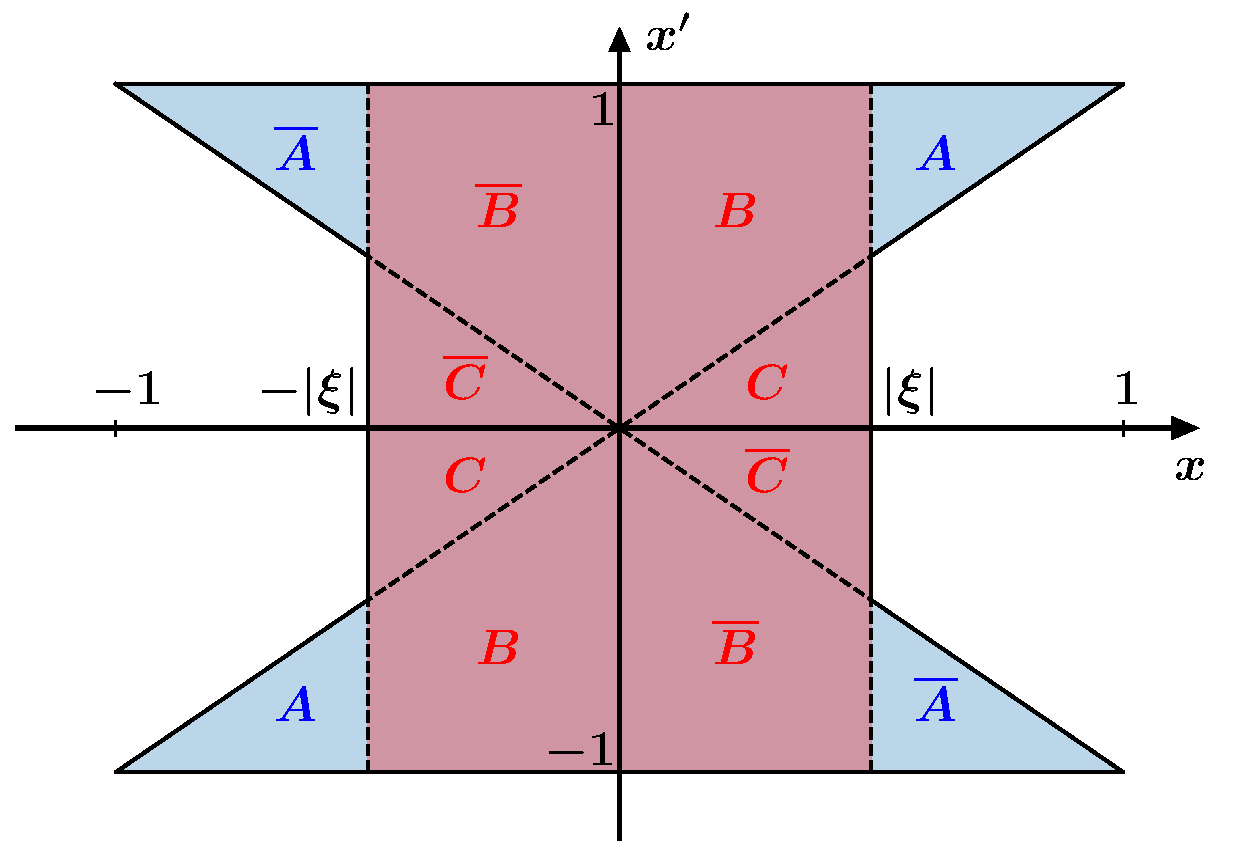
\includegraphics[width=0.7\textwidth]{plots/GPDIntDomain}
    \caption{Support domain of the evolution kernel
      $\mathbb{P}\left(\frac{x}{\xi},\frac{x'}{\xi}\right)$.\label{fig:GPDIntDomain}}
  \end{centering}
\end{figure}
Knowing the support of the evolution kernel, Eq.~(\ref{eq:eveq}) can
be rearranged as follows:
\begin{equation}
\displaystyle\mu^2\frac{d}{d\mu^2}f(\pm x,\xi) =\int_{b(x)}^{1}\frac{dx'}{x'}\left[\frac{x'}{\left|2\xi\right|}\mathbb{P}\left(\pm \frac{x}{\xi},\frac{x'}{\xi}\right)f(x',\xi)+\frac{x'}{\left|2\xi\right|}\mathbb{P}\left(\mp \frac{x}{\xi},\frac{x'}{\xi}\right)f(-x',\xi)\right]\,,
\end{equation}
with:
\begin{equation}\label{eq:lowintb}
b(x) = |x|\theta\left(\left|\frac{x}{\xi}\right|-1\right)\,,
\end{equation}
and where we have used the symmetry property of the evolution kernels
$\mathbb{P}(y,y')=\mathbb{P}(-y,-y')$. In the unpolarised case, it is useful to
define:\footnote{Notice the seemingly unusual fact that $f^{+}$ is
  defined as difference and $f^{-}$ as sum of GPDs computed at
  opposite values of $x$. This can be understood from the fact that,
  in the forward limit, $f(-x)= -\overline{f}(x)$, \textit{i.e.} the
  PDF of a quark computed at $-x$ equals the PDF of the corresponding
  antiquark computed at $x$ with opposite sign.}
\begin{equation}\label{eq:pmdef}
\begin{array}{rcl}
\displaystyle f^{\pm}(x,\xi) &=&\displaystyle  f(x,\xi) \mp
                       f(-x,\xi)\,,\\
\\
\displaystyle \mathbb{P}^{\pm}(y,y') &=&\displaystyle  \mathbb{P}(y,y') \mp \mathbb{P}(-y,y')\,,
\end{array}
\end{equation}
so that the evolution equation for $f^{\pm}$ reads:
\begin{equation}\label{eq:eveq2}
\displaystyle\mu^2\frac{d}{d\mu^2}f^{\pm}(x,\xi) = \int_{b(x)}^{1}\frac{dx'}{x'}\frac{x'}{\left|2\xi\right|}
                                                         \mathbb{P}^{\pm}\left(\frac{x}{\xi},\frac{x'}{\xi}\right)f^{\pm}(x',\xi)\,.
\end{equation}
In fact, the $f^{\pm}$ distributions are the GPD analogous of the
$\pm$ forward distributions that can then be used to construct the
usual singlet and non-singlet distributions in the QCD evolution
basis. This also determines the flavour structure of the evolution
kernels $\mathbb{P}^{\pm}$. Specifically, from now on we will
understand that $\mathbb{P}^+$ is a $2\times2$ matrix in flavour
space, while $\mathbb{P}^-$ is a flavour-scalar non-singlet evolution
kernel.

It is relevant to observe that the presence of the $\theta$-function
in the lower integration bound $b$, Eq.~(\ref{eq:lowintb}), is such
that for $|x|>|\xi|$ the evolution equation has the exact form of the
DGLAP evolution equation which corresponds to integrating over the
blue regions in Fig.~\ref{fig:GPDIntDomain} (henceforth DGLAP
region). Conversely, for $|x|\leq|\xi|$ the lower integration bound
becomes zero and the evolution equation assumes the form of the
so-called ERBL equation that describes the evolution of meson
distribution amplitudes (DAs). This corresponds to integrating over
the red region (henceforth ERBL region). Crucially, in the limits
$\xi\rightarrow 0$ and $\xi\rightarrow \pm1$ one recovers the DGLAP
and ERBL equations, respectively.

For later convenience, we define the parameter:
\begin{equation}
\kappa(x) = \frac{\xi}{x}\,,
\end{equation}
so that:
\begin{equation}
\frac{x'}{\left|2\xi\right|}
\mathbb{P}^{\pm}\left(\frac{x}{\xi},\frac{x'}{\xi}\right)={\rm sign}(\xi)\frac{1}{2\kappa}
\frac{x'}{x} \mathbb{P}^{\pm}\left(\frac{1}{\kappa},\frac{1}{\kappa}
  \frac{x'}{x}\right)\equiv {\rm sign}(\xi)\mathcal{P}^{\pm}\left(\kappa,\frac{x}{x'}\right)\,,
\end{equation}
where the last equality effectively defines the \textit{DGLAP-like}
splitting function:
\begin{equation}\label{eq:DGLAPevk}
  \mathcal{P}^{\pm}(\kappa,y) = \frac{1}{2\kappa y}
  \mathbb{P}^{\pm}\left(\frac{1}{\kappa},\frac{1}{\kappa y}\right)\,.
\end{equation}
Plugging this definition into the integral in the r.h.s. of
Eq.~(\ref{eq:eveq2}) and performing a change of variable gives:
\begin{equation}\label{eq:DGLAPforGPDs}
\displaystyle\mu^2\frac{d}{d\mu^2}f^{\pm}(x,\xi)= {\rm sign}(\xi)\int_{b(x)}^{1}\frac{dy}{y}\mathcal{P}^{\pm}\left(\kappa, \frac{x}{y}\right)f^{\pm}\left(y,\xi\right)={\rm sign}(\xi)\int_{x}^{x/b(x)}\frac{dy}{y}\mathcal{P}^{\pm}\left(\kappa,y\right)f^{\pm}\left(\frac{x}{y},\xi\right)\,,
\end{equation}
with:
\begin{equation}
b(x) = |x|\theta\left(\frac{1}{|\kappa|}-1\right)=|x|\theta\left(1-|\kappa|\right)\,,
\end{equation}
which (almost) has the form of a ``standard'' DGLAP equation. The only
difference is that the upper integration bound is not one but rather
$x/b(x)$ with $b(x)$. As discussed in the document
\textit{IntegralStructure.pdf}, this difference can be handled within
APFEL (up to a numerical approximation to be assessed) by adjusting
the integration procedure.

In the following we will assume $\xi>0$ as, so far, this is the only
experimentally accessible region. This allows us to get rid of
${\rm sign}(\xi)$ in Eq.~(\ref{eq:DGLAPforGPDs}). In addition, we can
also restrict to positive values of $x$ because negative values can be
easily accessed by symmetry using Eq.~(\ref{eq:pmdef}):
$f^{\pm}(-x,\xi)=\mp f^{\pm}(x,\xi)$.

\section{Anomalous dimensions}

A crucial ingredient for an efficient implementation of GPD evolution
is the availability of the DGLAP-like splitting functions
$\mathcal{P}^{\pm}$ defined in Eq.~(\ref{eq:DGLAPevk}) in a closed
form amenable to be easily integrated as in
Eq.~(\ref{eq:DGLAPforGPDs}).

In order to address this problem, we need to make the flavour
structure of the evolution kernels explicit. Working in the QCD
evolution basis, we have:
\begin{equation}
\mathcal{P}^+=\begin{pmatrix}
P_{qq}&P_{qg}\\
P_{gq}&P_{gg}
\end{pmatrix}\,,
\end{equation}
and:
\begin{equation}
\mathcal{P}^-=P^{\rm NS}\,,
\end{equation}
where $P^{\rm NS}$ is the appropriate evolution kernel. At one loop it
turns out that all the non-singlet splitting functions are equal
amongst and to $P_{qq}^{(0)}$, \textit{i.e.}
$P^{{\rm NS},(0)}=P_{qq}^{(0)}$.

The explicit form of the one-loop anomalous dimensions can be found,
for example, in Ref.~\cite{Blumlein:1999sc}. However, these functions
are tricky to integrate numerically due to the presence of
$\theta$-functions. In order to define the basic steps to reduce the
anomalous dimension to a suitable form, let us consider the
non-singlet unpolarised anomalous dimension at one loop. Using
Eq.~(\ref{eq:DGLAPevk}), one finds:
\begin{equation}\label{eq:GPDP0}
  P^{{\rm NS},(0)}(\kappa,y) =\left\{
\begin{array}{ll}
  \displaystyle
  2C_F\left[\frac{1+(1-2\kappa^2)y^2}{(1-y)(1-\kappa^2 y^2)}\right]_+\,,&\quad
                                                                 0\leq\kappa\leq
                                                                 1\,,\\
  \\
  \displaystyle
  2C_F\left[\frac{1}{1-y}+\frac12\frac{1-\kappa}{\kappa(1+\kappa y)}\right]_+\,,&\displaystyle \quad 1
                                   \leq\kappa\leq\frac{1}{x}\,.
\end{array}
\right.
\end{equation}
It is interesting to take the DGLAP limit at $\kappa\rightarrow 0$:
\begin{equation}
 P^{{\rm NS},(0)}(0,y) = 2C_F\left[\frac{1+y^2}{1-y}\right]_+\,,
\end{equation}
that coincides with the usual DGLAP splitting function.  While the
crossover point at $\kappa=1$ gives:
\begin{equation}\label{eq:pns0co}
  P^{{\rm NS},(0)}(1,y) = 2C_F\left[\frac{1}{1-y}\right]_+\,,
\end{equation}
regardless of whether the limit is taken from the DGLAP region
($\kappa\rightarrow 1^-$) of from the ERBL region
($\kappa\rightarrow 1^+$). This tells us that
$\mathcal{P}_{qq}^{+(0)}(\kappa,y)$ is a continuos function of
$\kappa$. Fig.~\ref{fig:GPDP0} displays the behaviour of the regular
part of the anomalous dimension $\mathcal{P}_{qq}^{+(0)}$ defined in
Eq.~(\ref{eq:GPDP0}) as a function of the parameter $\kappa$ for
different values of the variable $y$. This plot shows the continuity
of $\mathcal{P}_{qq}^{+(0)}$ at $\kappa=1$.
\begin{figure}[t]
  \begin{centering}
    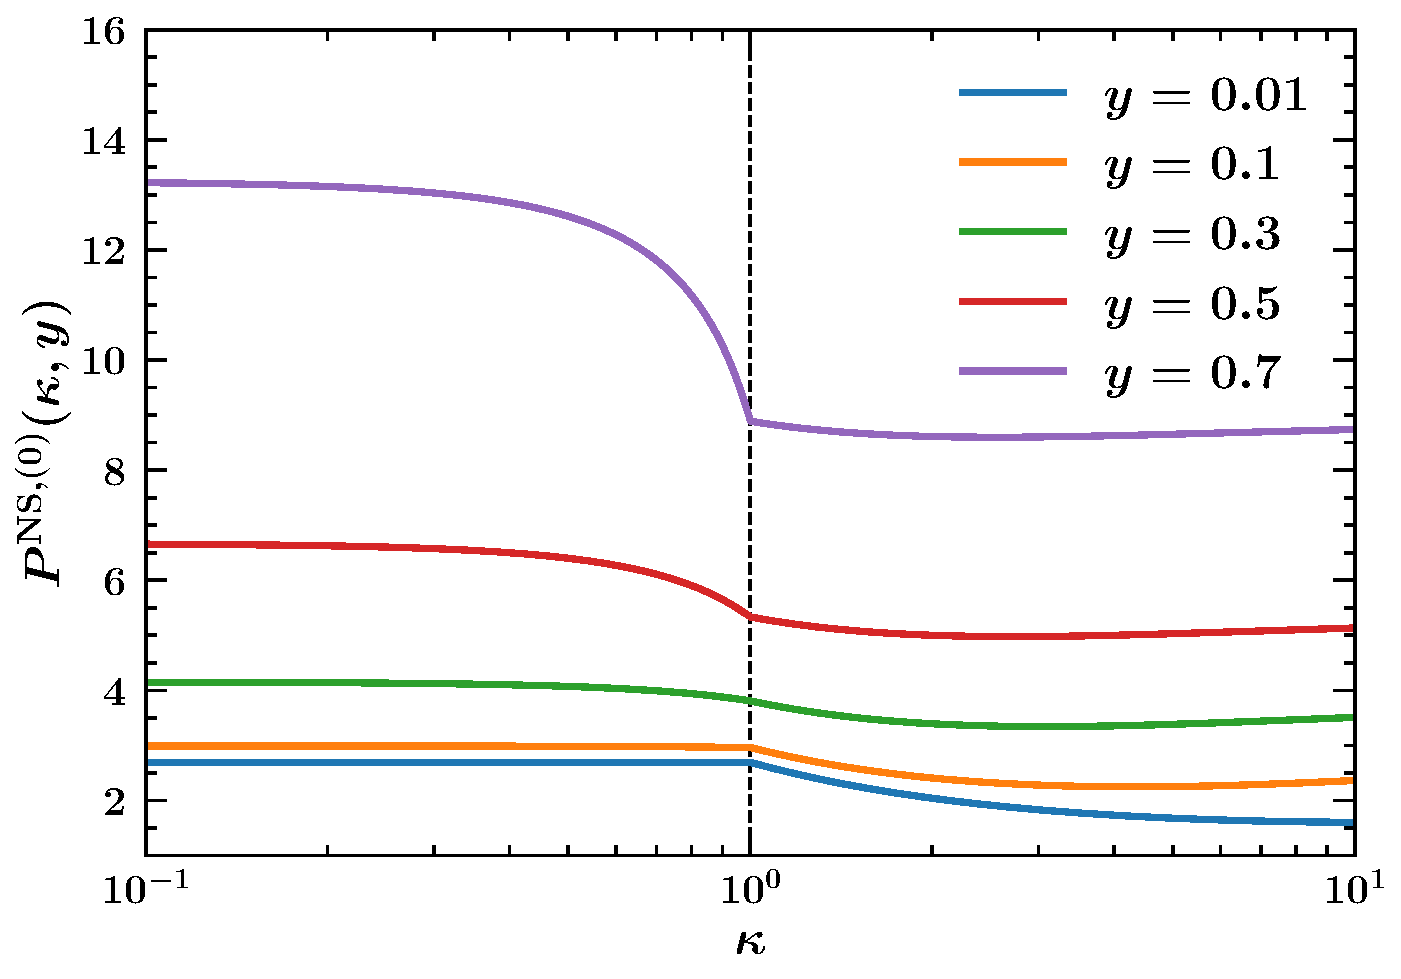
\includegraphics[width=0.6\textwidth]{plots/GPDP0}
    \caption{Behaviour of the anomalous dimension
      $P^{{\rm NS},(0)}$ as a function of $\kappa$ for
      different values of $y$.\label{fig:GPDP0}}
  \end{centering}
\end{figure}
Since $P_{qq}^{(0)}=P^{{\rm NS},(0)}$, what we discussed above applies
verbatim to $P_{qq}^{(0)}$.

Let us now turn to the remaining splitting functions $P_{qg}^{(0)}$,
$P_{gq}^{(0)}$, and $P_{gg}^{(0)}$. Their explicit expressions
read\footnote{The expression for $P_{gq}^{(0)}$ derived from
  Ref.~\cite{Blumlein:1999sc} seems to be wrong. I have derived the
  seemingly correct expression from Ref.~\cite{Ji:1996nm} by
  performing the replacement $\xi\rightarrow 2\kappa y$ in Eq.~(24).}:
\begin{equation}\label{eq:GPDP0qg}
  P_{qg}^{(0)}(\kappa,y) =\left\{
\begin{array}{ll}
  \displaystyle
  4 n_f T_R \frac{1 - 2y + (2 - \kappa^2) y^2}{(1 - \kappa^2 y^2)^2}\,,&\quad
                                                                 0\leq\kappa\leq
                                                                 1\,,\\
  \\
  \displaystyle 2n_f T_R \left[\frac{1 + \kappa}{\kappa^2 (1 + \kappa y)}\right] \left[\frac{1 - \kappa}{\kappa y }+\frac{1}{1 + \kappa y}\right]\,,&\displaystyle \quad 1
                                   \leq\kappa\leq\frac{1}{x}\,,
\end{array}
\right.
\end{equation}
\begin{equation}\label{eq:GPDP0gq}
  P_{gq}^{(0)}(\kappa,y) =\left\{
\begin{array}{ll}
  \displaystyle
2 C_F \left[\frac{2 - 2y + (1 - \kappa^2) y^2}{y (1 - \kappa^2 y^2)}\right]\,,&\quad
                                                                 0\leq\kappa\leq
                                                                 1\,,\\
  \\
\displaystyle  C_F \left[\frac{2(1+\kappa) - (1 - \kappa^2) y}{\kappa y (1 + \kappa y)}\right]\,,&\displaystyle \quad 1
                                   \leq\kappa\leq\frac{1}{x}\,,
\end{array}
\right.
\end{equation}
\begin{equation}\label{eq:GPDP0gg}
  P_{gg}^{(0)}(\kappa,y) =\left\{
\begin{array}{ll}
  \displaystyle
4 C_A\left[ \frac{-2 + y (1 - y + \kappa^2 (1 + y))}{(1 - \kappa^2 y^2)^2}+\frac{1}{y}+\frac1{\left(1-y\right)_+}\right]+\delta(1-x)\frac{11C_A-4n_fT_R}{3}\,,&\quad
                                                                 0\leq\kappa\leq
                                                                 1\,,\\
  \\
\displaystyle  C_A\left[\frac{-1 + 3 \kappa^2 - 
   \kappa (2 + (1 - \kappa)^2 \kappa) y}{\kappa^3 y (1 + \kappa y)^2}+\frac{2}{y}+\frac{2}{\left(1-y\right)_+}\right]+\delta(1-x)\frac{11C_A-4n_fT_R}{3}
\,,&\displaystyle \quad 1
                                   \leq\kappa\leq\frac{1}{x}\,.
\end{array}
\right.
\end{equation}
Their forward limit ($\kappa=0$) is:
\begin{equation}
\begin{array}{l}
  \displaystyle P_{qg}^{(0)}(0,y) = 4 n_f T_R \left[y^2+(1 - y)^2\right] \\
\\
  \displaystyle
P_{gq}^{(0)}(0,y) =2 C_F \left[\frac{1+(1 - y)^2}{y}\right]\,,\\
\\
  \displaystyle
  P_{gg}^{(0)}(0,y) =4 C_A\left[ -2 + y (1 - y)+\frac{1}{y}+\frac1{\left(1-y\right)_+}\right]+\delta(1-x)\frac{11C_A-4n_fT_R}{3}\,,
\end{array}
\end{equation}
which coincides with the usual one-loop DGLAP splitting functions. At
the crossover point $\kappa=1$ the evolution kernels reduce to:
\begin{equation}
  P_{qg}^{(0)}(1,y) = \frac{4 n_f T_R}{(1 + y)^2}\,,
\end{equation}
\begin{equation}
  P_{gq}^{(0)}(1,y) =\frac{4 C_F}{y (1 + y)}\,,
\end{equation}
\begin{equation}
  P_{gg}^{(0)}(1,y) =4 C_A\left[\frac{1+y^2}{y(1 + y)^2 \left(1-y\right)_+}\right]+\delta(1-y)\frac{11C_A-4n_fT_R}{3}\,.
\end{equation}
Interestingly, like $P^{{\rm NS},(0)}$ and $P_{qq}^{(0)}$ , also
$P_{qg}^{(0)}$, $P_{gq}^{(0)}$, and $P_{gg}^{(0)}$ are continuos in
$\kappa=1$.

\subsection{End-point (local) contributions}

Some of the expressions for the anomalous dimensions discussed above
contain a $+$-prescribed terms. It is important to treat these terms
properly accounting for additional local terms stemming from the
``incompleteness'' of the convolution integrals. More specifically,
the defintion of the $+$-prescription for the function $g$ (singular
in $y=1$) convoluted with a smooth test function $f$ is:
\begin{equation}
  \int_0^{1^+}
  dy\,\left[g(y)\right]_+f(y)=\int_0^{1^+} dy\,g(y)\left[f(y)-f(1)\right]\,.
\end{equation}
Now, we need to work out the action of the $+$-prescription on
integrals of the following kind (\textit{cfr.}
Eq.~(\ref{eq:DGLAPforGPDs})):
\begin{equation}\label{eq:divint}
I=\int_x^cdy\,\left[g(y)\right]_+f(y)\,,\quad x<1\quad\mbox{and}\quad c\geq 1\,.
\end{equation}
In order to apply the definition of $+$-prescription, we manipulate
the integral above as follows:
\begin{equation}\label{eq:explicitexpr}
\begin{array}{rcl}
I&=&\displaystyle
     \int_0^{1^+}dy\,\left[g(y)\right]_+f(y)-\int_0^xdy\,g(y)f(y)+\int_{1^+}^cdy\,g(y)f(y)\\
\\
&=&\displaystyle
    \int_0^{1^+}dy\,g(y)\left[f(y)-f(1)\right]-\int_0^xdy\,g(y)f(y)+\int_{1^+}^cdy\,g(y)f(y)\\

\\
&=&\displaystyle
    \int_x^{c}dy\,g(y)\left[f(y)-f(1)\right]+f(1)\left[L_1(x)+L_2(c)\right]
\end{array}
\end{equation}
where for shortness we have defined:
\begin{equation}
L_1(x)=-\int_0^xdy\,g(y) \quad\mbox{and}\quad L_2(c)=\int_{1^+}^cdy\,g(y)\,.\\
\end{equation}
The term $L_1$ is the usual term arising from the incompleteness of
the convolution integral and is finite for $x<1$. The term $L_2$ is
new.  In the DGLAP region ($\kappa<1$) the upper integration bound $c$
is equal to one so that $L_2(1)=0$ and we recover the usual DGLAP
structure. In the ERBL region ($\kappa>1$), instead, $c=+\infty$ so
that:
\begin{equation}
L_2(\infty)=\int_{1^+}^\infty dy\,g(y)\,.
\end{equation}
The question now is whether the second integral in the rightmost term
converges: the answer is generally not. A simple example is
Eq.~(\ref{eq:pns0co}) that, for $\kappa=1^+$ gives:
\begin{equation}
\int_{1^+}^\infty\frac{dy}{1-y} = -\infty\,.
\end{equation}
By inspection, one finds that this divergence is logarithmic,
signifying that the function $g$ goes to zero linearly as
$y\rightarrow \infty$. Of course, the presence of this divergence
seems to invalidate the full evolution procedures because the
derivative of GPDs with respect to $\mu$ in the ERBL region is not
defined. The question is how to overcome this problem. Since the
function $g$ is the result of a perturbative calculation, the only
possibility relies on imposing an appropriate constraint on test
function $f$ that guarantees the convergence of the integral in
Eq.~(\ref{eq:divint}). To do so, we need to \textit{require} that the
function $f$ is such that the last term in the r.h.s. of the first
line of Eq.~(\ref{eq:explicitexpr}) converges when $c=\infty$:
\begin{equation}
  \left|\int_{1^+}^\infty dy\,g(y)f(y)\right|<\infty\,.
\end{equation}
As we will see in the next section, the requirement of continuity of
GPDs sets the particular value of this integral at $x=\xi$ to zero.
Since $g$ decays linearly, in order for the integral to converge, also
the function $f$ needs to tend to zero as $y\rightarrow \infty$ as:
\begin{equation}
f(y)\mathop{\longrightarrow}_{y\rightarrow\infty}\frac1{y^a}\,,\quad a>0\,.
\end{equation}


\subsection{On continuity of GPDs}

It is well known that GPDs are required to be continuous at $x=\xi$
for factorisation to be valid~\cite{Radyushkin:1997ki}. It is thus
interesting to consider the consequence of this constraint. To this
end, let us consider the limits of Eq.~(\ref{eq:eveq2}) for
$x\rightarrow \xi^\pm$:
\begin{equation}\label{eq:limit1}
\lim_{x\rightarrow
  \xi^+}\displaystyle\mu^2\frac{d}{d\mu^2}f^{\pm}(x,\xi) =
\mu^2\frac{d}{d\mu^2}f^{\pm}(\xi,\xi)=\int_{\xi}^{1}\frac{dx'}{2\xi}
                                                         \mathbb{P}^{\pm}\left(\frac{\xi^+}{\xi},\frac{x'}{\xi}\right)f^{\pm}(x',\xi)\,,
\end{equation}
and:
\begin{equation}\label{eq:limit2}
\lim_{x\rightarrow \xi^-}\displaystyle\mu^2\frac{d}{d\mu^2}f^{\pm}(x,\xi) = \mu^2\frac{d}{d\mu^2}f^{\pm}(\xi,\xi)=\int_{0}^{1}\frac{dx'}{2\xi}
                                                         \mathbb{P}^{\pm}\left(\frac{\xi^-}{\xi},\frac{x'}{\xi}\right)f^{\pm}(x',\xi)\,,
\end{equation}
where we have used the continuity of $f^{\rm}$ at $x=\xi$. As we have
shown in the previous section, anomalous dimension at one loop are
also continuous in $x=\xi$ (\textit{i.e.} in $\kappa=1$), such that:
\begin{equation}
  \mathbb{P}^{\pm}\left(\frac{\xi^+}{\xi},y\right) =
  \mathbb{P}^{\pm}\left(\frac{\xi^-}{\xi},y\right) = \mathbb{P}^{\pm}\left(1,y\right)\,.
\end{equation}
Taking the difference between Eqs.~(\ref{eq:limit1})
and~(\ref{eq:limit2}) paying attention to remove also the end point
contributions, one finds, at least at one loop, that:
\begin{equation}
  \int_{0}^{\xi^-}\frac{dx'}{2\xi}\,\mathbb{P}^{\pm}\left(1,\frac{x'}{\xi}\right)f^{\pm}(x',\xi) =\int_{0}^{\xi^-}\frac{dx'}{x'}\,\mathcal{P}^{\pm}\left(1,\frac{\xi}{x'}\right)f^{\pm}(x',\xi) =\int_{1^+}^{\infty}\frac{dx'}{x'}\,\mathcal{P}^{\pm}\left(1,x'\right)f^{\pm}\left(\frac{\xi}{x'},\xi\right)=0\,.
\end{equation}
This appears to be some sort of sum rule that the GPDs and anomalous
dimensions in the ERBL region have to fullfil. We will attempt a
numerical estimate of the impact of possible violations of this
requirement.

\section{On Vinnikov's code}

The purpose of this short note is to draw the attention on a possible
incongruence of the GPD evolution code developed by Vinnikov and
presented in Ref.~\cite{Vinnikov:2006xw}. For definiteness, we
concentrate on the non-singlet $H_{\rm NS}$ GPD in the DGLAP region
$x>\xi$, whose evolution equation is given in Eq.~(29). For
completeness, I report that equation here:
\begin{equation}\label{eq:Vinnikov}
\begin{array}{rcl}
\displaystyle \frac{d H_{\rm NS}(x,\xi,Q^2)}{d\ln
  Q^2}&=&\displaystyle\frac{2\alpha_s(Q^2)}{3\pi}\Bigg[\int_x^1 dy
          \frac{x^2+y^2-2\xi^2}{(y-x)(y^2-\xi^2)}\left(H_{\rm
          NS}(y,\xi,Q^2)-H_{\rm NS}(x,\xi,Q^2)\right)\\
\\
&+&\displaystyle H_{\rm
    NS}(x,\xi,Q^2)\bigg(\frac32+2\ln(1-x)+\frac{x-\xi}{2\xi}\ln((x-\xi)(1+\xi))\\
\\
&-&\displaystyle \frac{x+\xi}{2\xi}\ln((x+\xi)(1-\xi))\bigg)\Bigg]\,.
\end{array}
\end{equation}
The limit for $\xi\rightarrow 0$ of the equation above should
reproduce the usual DGLAP evolution equation:
\begin{equation}
\displaystyle \frac{d H_{\rm 
NS}(x,0,Q^2)}{d\ln
  Q^2}=\frac{\alpha_s(Q^2)}{4\pi}\int_x^1 \frac{dz}{z}\left[\hat{P}_{\rm
  NS}\left(z\right)\right]_+H_{\rm NS}\left(\frac{x}{z},0,Q^2\right)\,,
\end{equation}
where:
\begin{equation}
\hat{P}_{\rm NS}\left(z\right)=2C_F\frac{1+z^2}{1-z}=2C_F\left[\frac{2}{1-z}-(1+z)\right]\,,
\end{equation}
with $C_F=4/3$. Written explicitly:
\begin{equation}\label{eq:DGLAPexpl}
\begin{array}{rcl}
  \displaystyle \frac{d H_{\rm NS}(x,0,Q^2)}{d\ln
    Q^2}&=&\displaystyle \frac{\alpha_s(Q^2)}{4\pi}2C_F\Bigg[\int_x^1 dz\,\frac{2}{1-z}\left(\frac1z H_{\rm NS}\left(\frac{x}{z},0,Q^2\right)-H_{\rm
      NS}(x,0,Q^2)\right)\\
\\
&-&\displaystyle \int_x^1 \frac{dz}{z}\, (1+z) H_{\rm
    NS}\left(\frac{x}{z},0,Q^2\right)\\
\\
 &+&\displaystyle H_{\rm NS}(x,0,Q^2)\left(\frac{3}{2}+2\ln(1-x)\right)\Bigg]\,.
\end{array}
\end{equation}
Now I explicitly take the limit for $\xi\rightarrow 0$ of
Eq.~(\ref{eq:Vinnikov}). The result is:
\begin{equation}
\begin{array}{rcl}
\displaystyle \frac{d H_{\rm NS}(x,0,Q^2)}{d\ln
  Q^2}&=&\displaystyle\frac{2\alpha_s(Q^2)}{3\pi}\Bigg[\int_x^1 dy
          \frac{x^2+y^2}{y^2 (y-x)}\left(H_{\rm
          NS}(y,0,Q^2)-H_{\rm NS}(x,0,Q^2)\right)\\
\\
&+&\displaystyle H_{\rm
    NS}(x,0,Q^2)\left(\frac32+2\ln(1-x)\right)\Bigg]\,.
\end{array}
\end{equation}
Some further simple algebraic manipulation finally gives:
\begin{equation}
\begin{array}{rcl}
\displaystyle \frac{d H_{\rm NS}(x,0,Q^2)}{d\ln
  Q^2}&=&\displaystyle\frac{\alpha_s(Q^2)}{4\pi}2C_F\Bigg[\int_x^1 dz\, 
          \frac{2}{1-z}\left(\frac{1}{z}H_{\rm
          NS}\left(\frac{x}{z},0,Q^2\right)-H_{\rm NS}(x,0,Q^2)\right)\\
\\
&-&\displaystyle \int_x^1 \frac{dz}{z}\,(1+z)H_{\rm
          NS}\left(\frac{x}{z},0,Q^2\right)\\
\\
&+&\displaystyle H_{\rm
    NS}(x,0,Q^2) \left(\frac32+2\ln(1-x)+\ln(x)+(1-x)\right)\Bigg]\,,
\end{array}
\end{equation}
that is close to the correct results, Eq.~(\ref{eq:DGLAPexpl}), except
for the two additional terms in the third line. Since the
$\xi\rightarrow 0$ limit does not seem to produce the correct result,
this suggests that the evolution code presented in
Ref.~\cite{Vinnikov:2006xw} may not be entirely correct.\footnote{It
  is, in fact, possible to correct Eq.~(\ref{eq:Vinnikov}) in such a
  way that its $\xi\rightarrow 0$ limit gives the correct DGLAP
  evolution equation.}

\newpage

\begin{thebibliography}{alp}

%\cite{Diehl:2003ny}
\bibitem{Diehl:2003ny}
  M.~Diehl,
  %``Generalized parton distributions,''
  Phys.\ Rept.\  {\bf 388} (2003) 41
  doi:10.1016/j.physrep.2003.08.002, 10.3204/DESY-THESIS-2003-018
  [hep-ph/0307382].
  %%CITATION = doi:10.1016/j.physrep.2003.08.002, 10.3204/DESY-THESIS-2003-018;%%
  %1016 citations counted in INSPIRE as of 30 Oct 2019

%\cite{Blumlein:1999sc}
\bibitem{Blumlein:1999sc}
  J.~Blumlein, B.~Geyer and D.~Robaschik,
  %``The Virtual Compton amplitude in the generalized Bjorken region: twist-2 contributions,''
  Nucl.\ Phys.\ B {\bf 560} (1999) 283
  doi:10.1016/S0550-3213(99)00418-6
  [hep-ph/9903520].
  %%CITATION = doi:10.1016/S0550-3213(99)00418-6;%%
  %86 citations counted in INSPIRE as of 13 Feb 2020

%\cite{Radyushkin:1997ki}
\bibitem{Radyushkin:1997ki}
A.~V.~Radyushkin,
%``Nonforward parton distributions,''
Phys. Rev. D \textbf{56} (1997), 5524-5557
doi:10.1103/PhysRevD.56.5524
[arXiv:hep-ph/9704207 [hep-ph]].
%1104 citations counted in INSPIRE as of 02 Jul 2020

%\cite{Ji:1996nm}
\bibitem{Ji:1996nm}
X.~D.~Ji,
%``Deeply virtual Compton scattering,''
Phys. Rev. D \textbf{55} (1997), 7114-7125
doi:10.1103/PhysRevD.55.7114
[arXiv:hep-ph/9609381 [hep-ph]].
%1183 citations counted in INSPIRE as of 08 Jul 2020

%\cite{Vinnikov:2006xw}
\bibitem{Vinnikov:2006xw}
A.~V.~Vinnikov,
%``Code for prompt numerical computation of the leading order GPD evolution,''
[arXiv:hep-ph/0604248 [hep-ph]].
%21 citations counted in INSPIRE as of 20 Jul 2020

\end{thebibliography}

\end{document}
